\documentclass{article}
\usepackage[utf8]{inputenc}
\usepackage{amsmath}
\usepackage{amsfonts}
\usepackage{tikz}
\usepackage{tkz-euclide}

\begin{document}

\begin{center}
    \section*{Maths Problems Set 1 (13 December 2019)}
\end{center}

\begin{enumerate}
    \item
    Each side length of the equilateral triangle below is 1. Find the area of the inscribed square.\\
    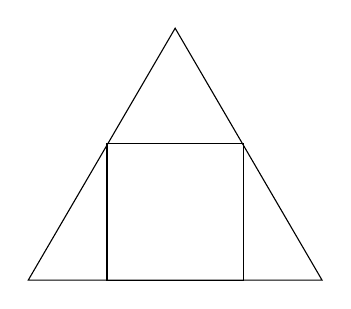
\begin{tikzpicture}
        \draw (-1.866, 0) -- (1.866, 0) -- (0, 3.2) -- cycle;
        \draw (-0.866, 0) -- (-0.866, 1.732) -- (0.866, 1.732) -- (0.866, 0) -- cycle;
    \end{tikzpicture}
    
    \item
    Initially there are $m$ balls in one bag, and $n$ in the other, where $m, n > 0$. Two different operations are allowed:
    \begin{enumerate}
        \item Remove an equal number of balls from each bag;
        \item Double the number of balls in one bag.
    \end{enumerate}
    Is it always possible to empty both bags after a finite sequence of operations?\\\\
    Operation (b) is now replaced with\\\\
    (b') Triple the number of balls in one bag.\\\\
    Is it now always possible to empty both bags after a finite sequence of operations?
    
    \item
    Prove that there are infinitely many non-trivial Pythagorean triples, i.e. not a multiple of a different Pythagorean triple.
    
    \item
    Straight lines are drawn on a infinite 2D plane. Show that the resulting regions can be coloured with two colors such that no adjacent regions have the same color.
    
    \item
    For a four digit number $n$ (using at least two different digits with leading zeros allowed), the digits of $n$ are rearranged to form the largest possible four digit number $a$ and the smallest possible four digit numbers $b$ (with leading zeros if necessary). The difference between the $a$ and $b$ is found, and this process is repeated with $n$ being this difference.\\
    \\
    Prove that the process eventually hits 6174 and remains there in at most 7 iterations for any four digit number $n$.
    
    \item
    Gnomes have friendships. Friendship is commutative. A gnome is odd if it has an odd number of friends. Show that there is always an even number of odd gnomes.
    
    \item
    Prove that if $A$ and $B$ are coprime where $A,B \in \mathbb{Z}$, then $\exists \text{ } s,t \in \mathbb{Z}$ such that $As+Bt=1$.
    
    \item
    Evaluate $\int_{0}^{1} \frac{1}{x+\sqrt{1-x^2}}  \text{ } \mathrm{d}x$.
    
    \item
    Find the smallest $a \geq 1$ such that $e^{y - x} \geq \frac{a + \sin x}{a + \sin y}$ for all $y \geq x$.
    
    \item
    $
        \text{Evaluate } \lim\limits_{n\to\infty} (\frac{1}{n+1} + \frac{1}{n+2} + \cdot \cdot \cdot + \frac{1}{2n})\text{.}
    $
    
    
    \item
    $
        \text{Find an expression for} \int_{1}^{n} (-1)^{\lfloor x \rfloor} \lfloor x \rfloor^{-1} \text{ } \mathrm{d}x \text{ where } n \in \mathbb{N}.
    $
    
    \item
    Prove that every prime has infinitely many multiples in the Fibonacci sequence. Prove that they have a constant frequency. Deduce that there are infinitely many Fibonacci numbers that are the product of only primes that had not previously occurred.
    
    \item
    Find all solutions to the Diophantine equation $4x^2 = y^3 + 1$.
    
    \item 
    Let $A = \{0, 1, ..., 2^n - 1, 2^n\}$ and $B = \{0, ..., n \}$. How many functions $g$ can be defined from $A$ to $B$ such that both of the following conditions hold:
    \begin{itemize}
        \item for all $x \in B$ we have $g(2^x) = x$
        \item for all $y, z \in A$ with $y \leq z$ we have $g(y) \leq g(z)$
    \end{itemize}
    
    
    \item
    Find all functions $f: \mathbb{Z} \to \mathbb{Z}$ such that for all $a,b \in \mathbb{Z}$:
    \begin{enumerate}
        \item $f(a)+f(b) = f(f(a+b))$, or
        \item $f(a)+f(2b) = f(f(a+b))$, or
        \item $f(a)+2f(b) = f(f(a+b))$
    \end{enumerate}
    
    \item
    There are $n$ points on 2D plane. Show that it is always possible to select at least $\sqrt{n}$ of this points so that the points selected do not form any equilateral triangles.
\end{enumerate}



\end{document}
